\documentclass[UTF8,a4paper,12pt]{ctexart}
\usepackage{thesis-style}
\usepackage{amsmath}

\graphicspath{{assets/}{../../outputs/experiment1/}}
\headermark{《金融经济数据挖掘》实验报告}
\reporttitle{《金融经济数据挖掘》实验报告}
\reportsubtitle{金融新闻情绪量化、羊群效应构建与非线性预测分析}
\author{丁致宇}
\studentid{202331060205}
\major{数据科学与大数据技术}
\phone{18765788600}
\date{2026年6月}

\begin{document}

\maketitle

\begin{ustcabstract}
本报告围绕《金融经济数据挖掘》实验指导书中金融非结构化数据处理与市场情绪建模任务展开。实验一完成金融新闻文本读取、清洗、去重、交易日过滤和 BERT 三分类情感标注，并按每 5 个沪深300交易日聚合生成周度情绪指标；实验二基于周度正负情绪比例构造情绪偏离度、观点分歧度和综合羊群效应指数；实验三将羊群效应指标与沪深300周收益率对齐，构造无未来信息泄露的滞后特征和滚动统计特征，使用 LightGBM 完成非线性时序预测、特征重要性分析、SHAP 解释和双向传导验证。

实验共处理原始金融新闻 60000 条，筛选、去空、去重并剔除非交易日新闻后，进入情绪标注的样本为 30623 条，样本交易日区间为 2014-10-08 至 2015-10-21。最终生成 51 行周度情绪指标、51 行羊群效应指标、50 行市场对齐数据和 45 行机器学习特征数据。正向模型（羊群效应预测收益率）测试集 $R^2=-0.2759$，说明样本外预测效果仍弱于均值基准；反向模型（收益率预测羊群效应）测试集 $R^2=0.0221$，IC 为 0.7333，方向命中率为 77.78\%，显示收益变化对后续舆情羊群强度具有更强的引导信号。总体而言，本实验完成了从非结构化金融文本到结构化情绪因子、羊群效应指标和非线性预测建模的完整工程链路，同时也表明在当前样本规模下，市场收益对情绪的反馈强于情绪对收益的先行预测。
\end{ustcabstract}
\keywords{金融文本挖掘；BERT；市场情绪；羊群效应；LightGBM；SHAP；金融反身性}

\clearpage
\tableofcontents
\clearpage

\section{实验要求理解与总体设计}

实验指导书以“金融非结构化数据预处理”为起点，但三个实验之间存在明确的数据依赖关系：实验一输出周度情绪指标，实验二在此基础上构建羊群效应指数，实验三再将羊群效应指数与沪深300指数收益率对齐并完成预测建模。因此，本报告采用一个完整实验链路统一呈现，同时在正文中分别对应实验一、实验二和实验三的要求。

本次实验的核心目标包括三点。第一，将金融新闻文本这类非结构化数据转化为可建模的结构化周度情绪指标；第二，依据情绪偏离和观点一致性构造羊群效应指数；第三，使用时序机器学习方法检验羊群效应与市场收益之间的预测关系和双向传导关系。为保证结果可复现，全部代码集中在 \path{experiment1/} 目录，原始数据位于 \path{data/experiment1/}，运行结果统一输出至 \path{outputs/experiment1/}。

\subsection{数据与输出口径}

实验使用两类老师配套数据：一是金融新闻文本数据，字段包括新闻编号、标题、正文、分词内容和发布时间；二是沪深300日度价格指数数据，用于构造交易日历和计算周收益率。新闻筛选区间设置为 2014-10-01 至 2015-10-31。周度统计单位不是普通自然周，而是按沪深300交易日历每 5 个交易日形成一组，从而避免周末和节假日造成的非交易日错位。

\begin{table}[H]
    \centering
    \caption{数据处理审计摘要}
    \label{tab:data-audit}
    \begin{tabular}{lr}
        \toprule
        项目 & 数值 \\
        \midrule
        原始新闻行数 & 60000 \\
        日期范围与正文非空过滤后行数 & 36181 \\
        正文重复删除行数 & 1705 \\
        剔除非交易日或交易日历外新闻行数 & 3853 \\
        最终进入情绪标注的交易日新闻行数 & 30623 \\
        样本交易日范围 & 2014-10-08 至 2015-10-21 \\
        情绪标注方法 & BERT 本地推理 \\
        周度情绪表行数 & 51 \\
        建模对齐数据行数 & 50 \\
        特征工程有效样本行数 & 45 \\
        \bottomrule
    \end{tabular}
\end{table}

\subsection{程序结构}

实验代码按职责拆分为多个模块。\path{config.py} 保存路径和参数，\path{data.py} 负责数据读取、清洗、交易日历构造、周度聚合和 SQLite 入库，\path{sentiment.py} 负责 BERT 情绪标注和词典回退方案，\path{analysis.py} 负责羊群效应构建、特征工程、LightGBM 建模和指标计算，\path{plots.py} 负责可视化，\path{main.py} 串联完整流程。完整源码见附录。

这种拆分方式可以减少单一脚本过长造成的维护困难，也便于逐步检查每个实验环节是否满足要求。运行入口为：

\begin{CodeBlock}
python -m experiment1.main
\end{CodeBlock}

\section{实验一：金融新闻文本预处理与周度情绪量化}

\subsection{数据清洗流程}

实验一首先读取 \texttt{新闻数据.xls}，将发布时间字段转换为标准时间格式，然后按实验要求筛选 2014 年 10 月至 2015 年 10 月的新闻。清洗过程包括三步：删除发布时间或正文为空的样本，按正文内容去除重复新闻，使用沪深300交易日历剔除非交易日新闻。这样处理的原因是：空文本无法做情绪推理，重复新闻会放大某些情绪信号，非交易日新闻则难以与当日市场价格严格对齐。

清洗后，新闻按照交易日历中的 \texttt{week\_id} 聚合。每个 \texttt{week\_id} 对应连续 5 个沪深300交易日，最终周度日期采用该组最后一个交易日作为 \texttt{week} 字段。该口径与后续沪深300周收益率计算保持一致。

\subsection{BERT 情感标注}

情绪标注使用本地 HuggingFace 模型 \path{yiyanghkust/finbert-tone-chinese}。模型标签映射为 Neutral $\rightarrow 0$、Positive $\rightarrow 1$、Negative $\rightarrow -1$，与本实验的正面、中性、负面三分类要求一致。程序优先使用 BERT 批量推理；当本地模型不可用时，才回退到金融情绪词典打分器。当前运行结果显示实际使用方法为 BERT。

将标题和正文拼接后输入模型，可以同时利用标题中的事件摘要和正文中的细节信息。推理时设置最大长度为 256，以控制长文本对显存和推理速度的影响。BERT 标注完成后，程序保留前 1000 条样本作为 \path{sentiment_labeled_sample.csv} 和数据库样例表，便于检查标注结果。

\subsection{周度情绪指标}

实验一要求输出 \texttt{WeekPositive}、\texttt{WeekNeutral}、\texttt{WeekNegative} 和周情绪占比 $P_t$。本实验严格按指导书公式计算：

\begin{equation}
P_t=\frac{WeekPositive_t}{WeekPositive_t+WeekNegative_t}.
\end{equation}

中性新闻参与 \texttt{WeekNeutral} 统计，但不进入 $P_t$ 的分母。这样处理能够突出正负方向性情绪，而不是让大量中性公告稀释乐观/悲观比例。

\begin{figure}[H]
    \centering
    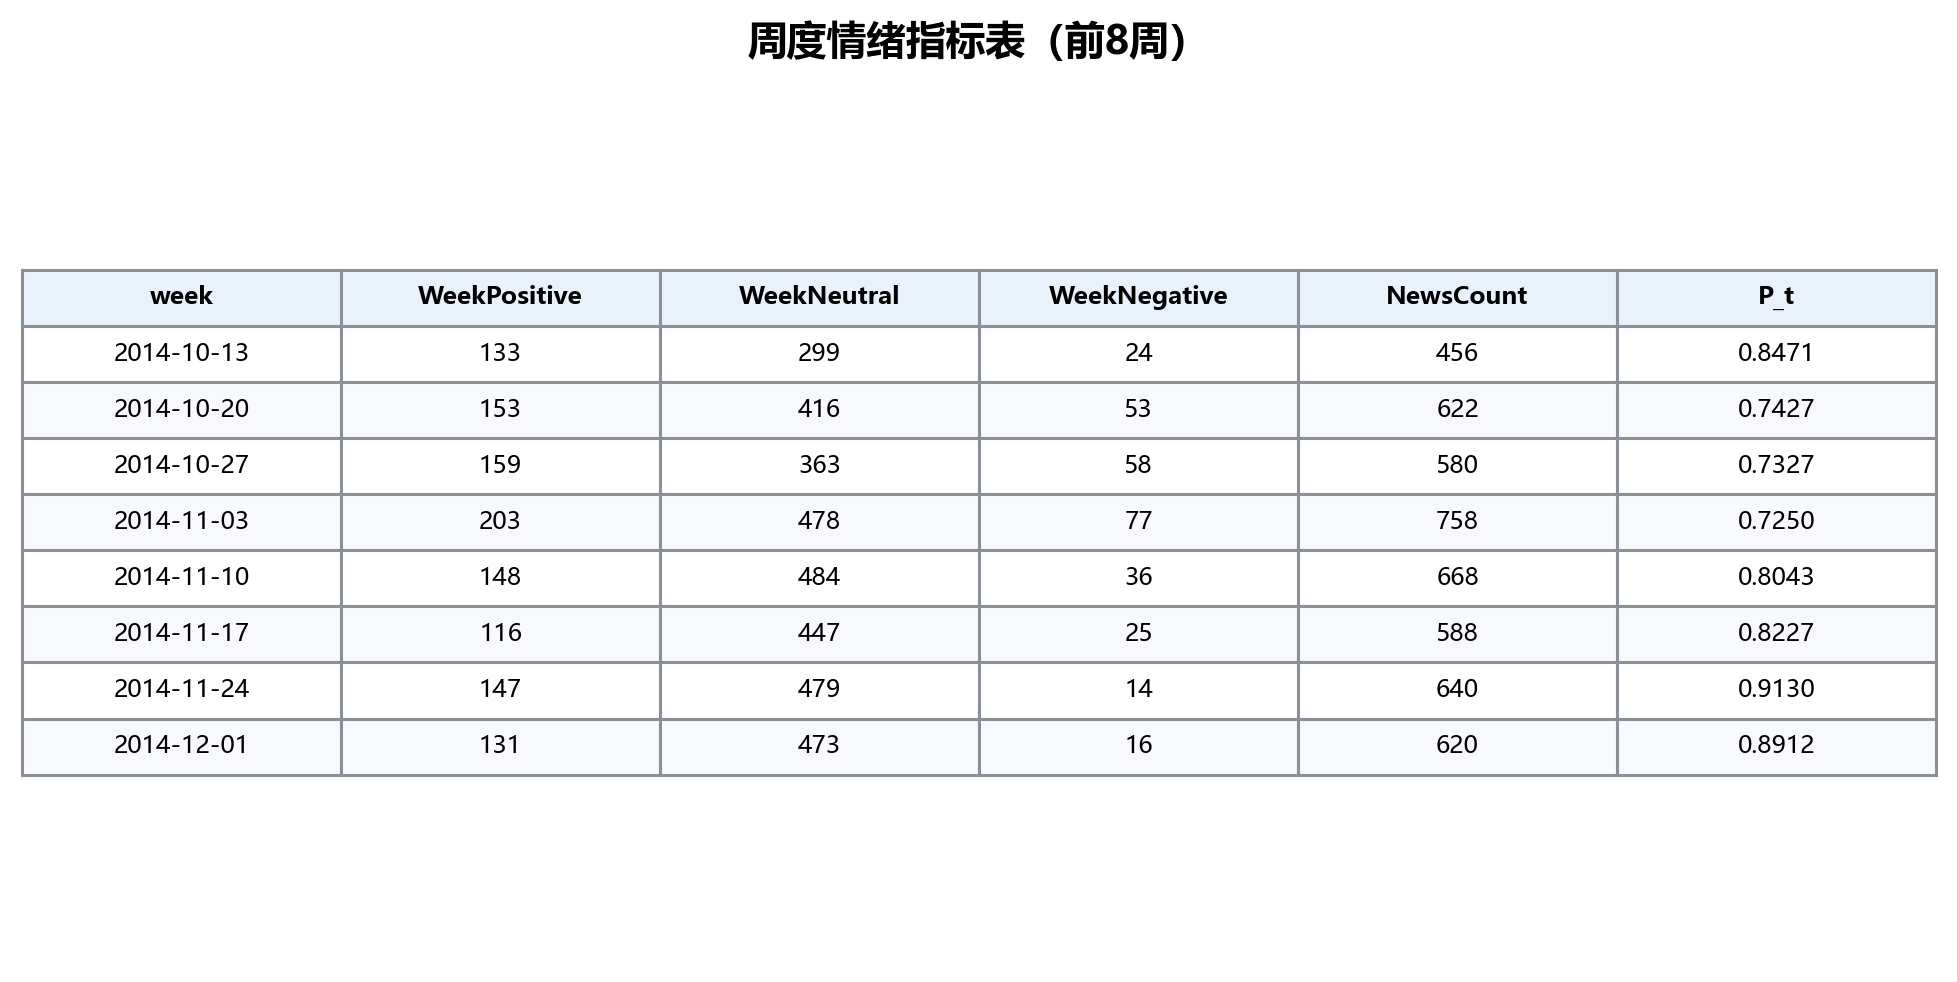
\includegraphics[width=0.98\textwidth]{weekly_sentiment_snapshot.png}
    \caption{周度情绪指标表截图}
    \label{fig:weekly-sentiment-snapshot}
\end{figure}

\begin{figure}[H]
    \centering
    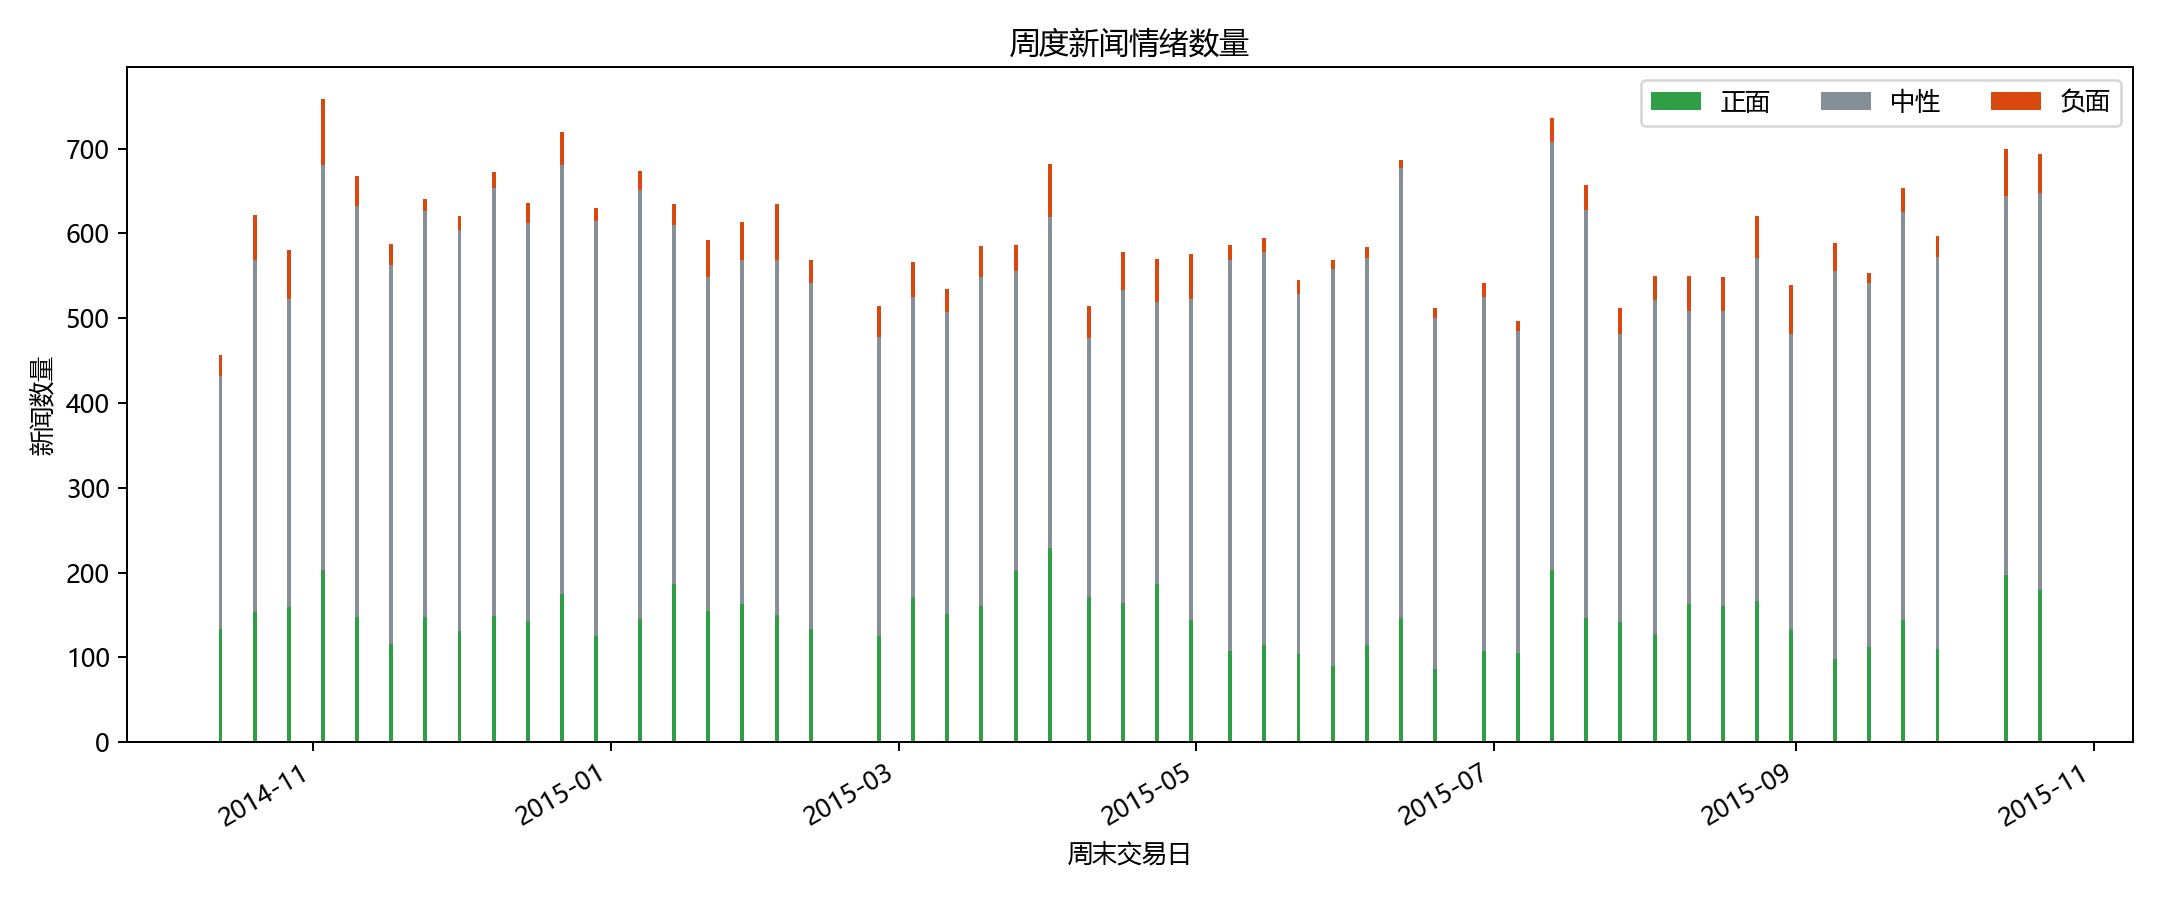
\includegraphics[width=0.92\textwidth]{weekly_sentiment_counts.png}
    \caption{周度新闻情绪数量堆叠图}
    \label{fig:weekly-sentiment-counts}
\end{figure}

从图 \ref{fig:weekly-sentiment-snapshot} 可见，周度情绪表包含实验要求的核心字段，并额外保留周起止日期、交易周编号和新闻总量，便于审计分组口径。图 \ref{fig:weekly-sentiment-counts} 显示，中性新闻数量整体较高，正面新闻数量通常高于负面新闻，说明新闻文本中存在明显的中性公告和偏正面信息披露特征。

\subsection{数据库存储结果}

实验一要求将周度情绪表存入数据库并导出 CSV。本实验使用 SQLite 数据库 \path{outputs/experiment1/experiment1.db} 保存关键结果，包括情绪样例、周度情绪、羊群指标、沪深300周收益和建模对齐数据。

\begin{figure}[H]
    \centering
    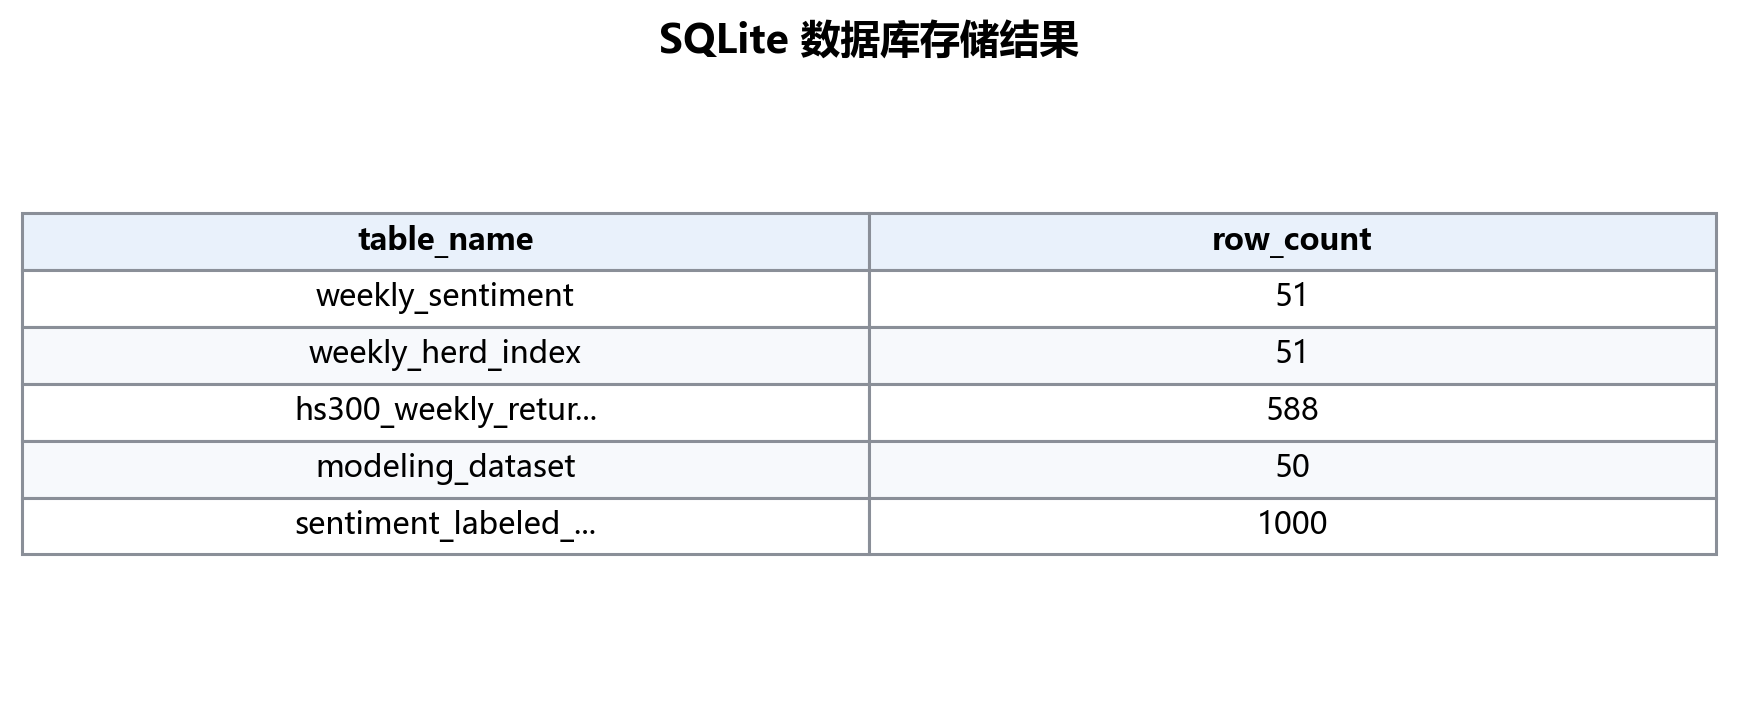
\includegraphics[width=0.72\textwidth]{database_snapshot.png}
    \caption{SQLite 数据库存储结果截图}
    \label{fig:database-snapshot}
\end{figure}

图 \ref{fig:database-snapshot} 表明，周度情绪表共有 51 行，与导出的 CSV 行数一致；羊群指标表同样为 51 行；建模对齐表在剔除首期历史基准缺失和收益率缺失后保留 50 行。

\section{实验二：羊群效应指标构建}

\subsection{指标构建逻辑}

实验二的任务是基于周度情绪指标构造羊群效应指数。单纯的乐观比例 $P_t$ 只能说明当周正面情绪占比，并不能直接表示羊群效应。真正的羊群行为应同时满足两个条件：其一，当周情绪相对历史水平出现明显偏离；其二，市场观点呈现单边一致，而不是多空均衡。

因此，本实验构造三个指标。首先，用过去 4 周 $P_t$ 均值作为正常情绪基准：

\begin{equation}
E(P_t)=\frac{1}{4}\sum_{i=1}^{4}P_{t-i}.
\end{equation}

其次，构造情绪偏离度：

\begin{equation}
H1_t=P_t-E(P_t).
\end{equation}

再次，构造观点分歧度：

\begin{equation}
H2_t=1-\frac{|WeekPositive_t-WeekNegative_t|}{WeekPositive_t+WeekNegative_t}.
\end{equation}

需要注意的是，按该定义，$H2_t$ 越小表示正负观点越单边，羊群一致性越强；$H2_t$ 越大表示正负观点越均衡，分歧越强。因此，最终综合指标采用情绪偏离强度与单边一致性相乘：

\begin{equation}
H3_t=Norm(|H1_t|)\times(1-Norm(H2_t)).
\end{equation}

其中 $Norm(\cdot)$ 表示 Min-Max 归一化。该实现与“情绪反常且观点一边倒时羊群效应更强”的金融逻辑一致。

\subsection{羊群效应指标结果}

\begin{figure}[H]
    \centering
    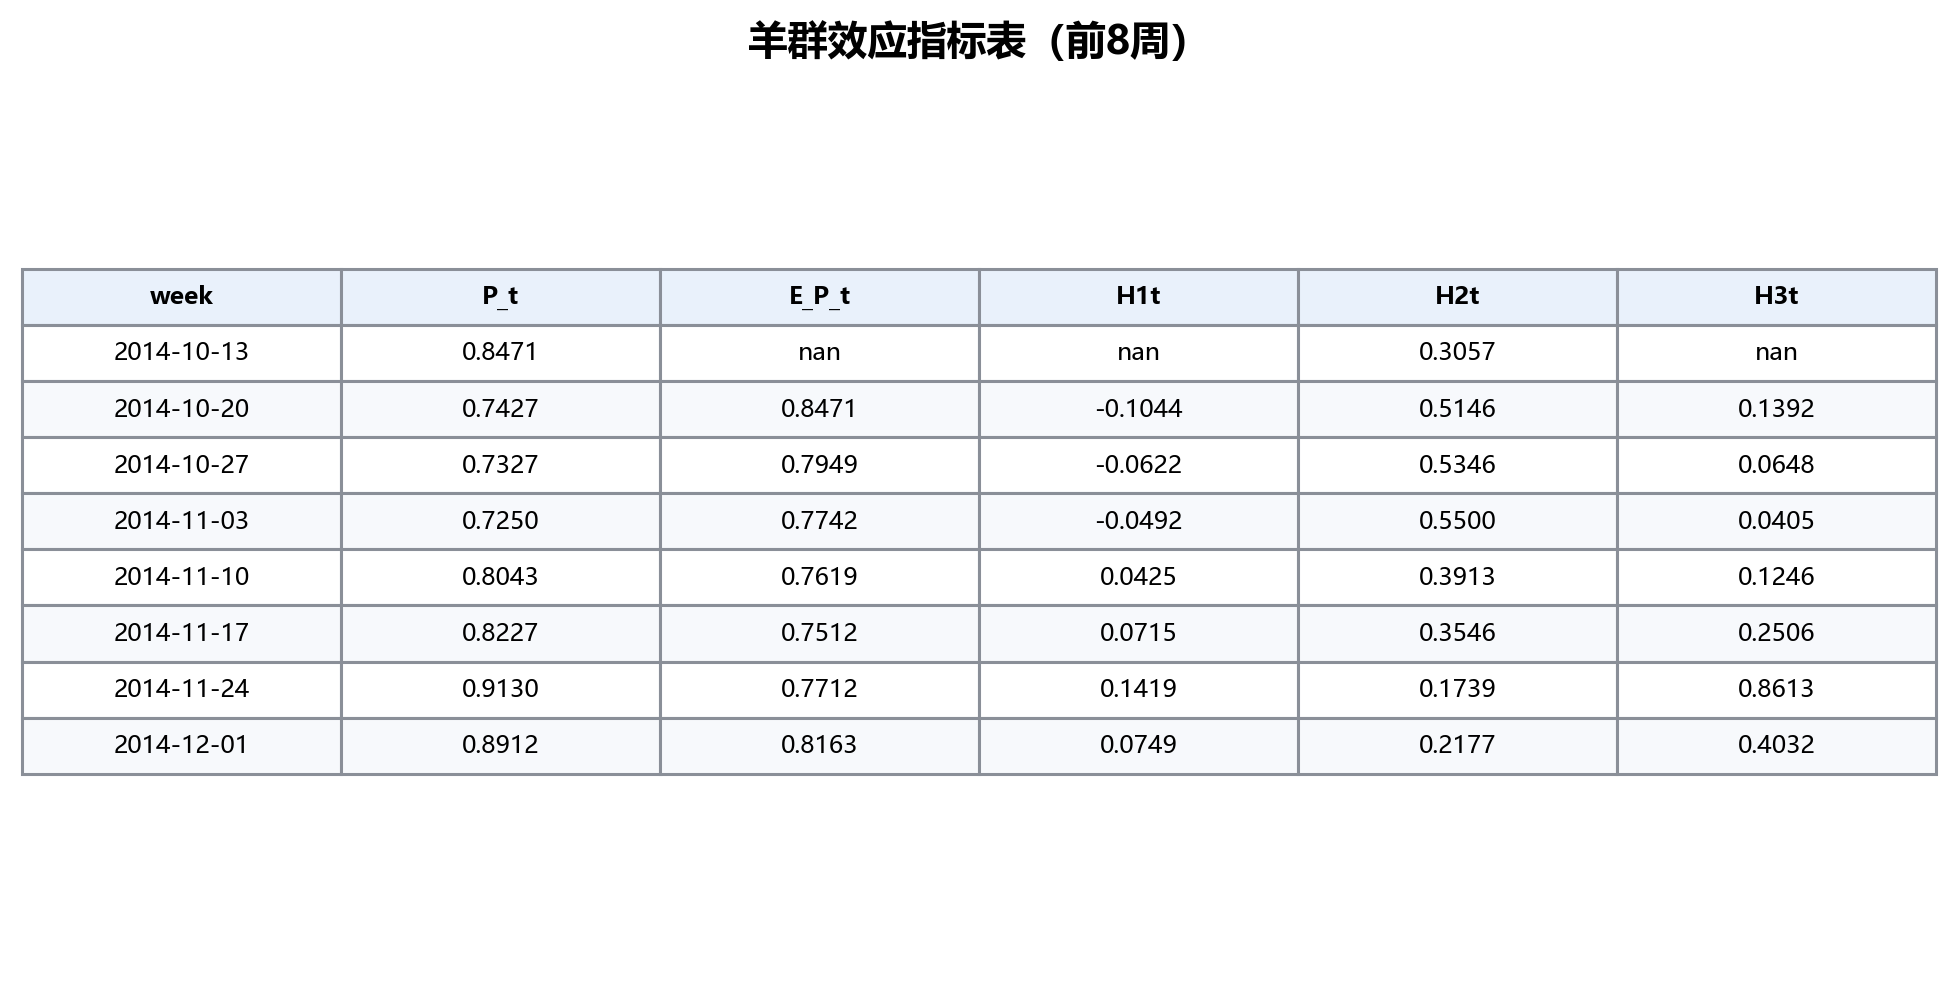
\includegraphics[width=0.98\textwidth]{herd_index_snapshot.png}
    \caption{羊群效应指标表截图}
    \label{fig:herd-index-snapshot}
\end{figure}

\begin{figure}[H]
    \centering
    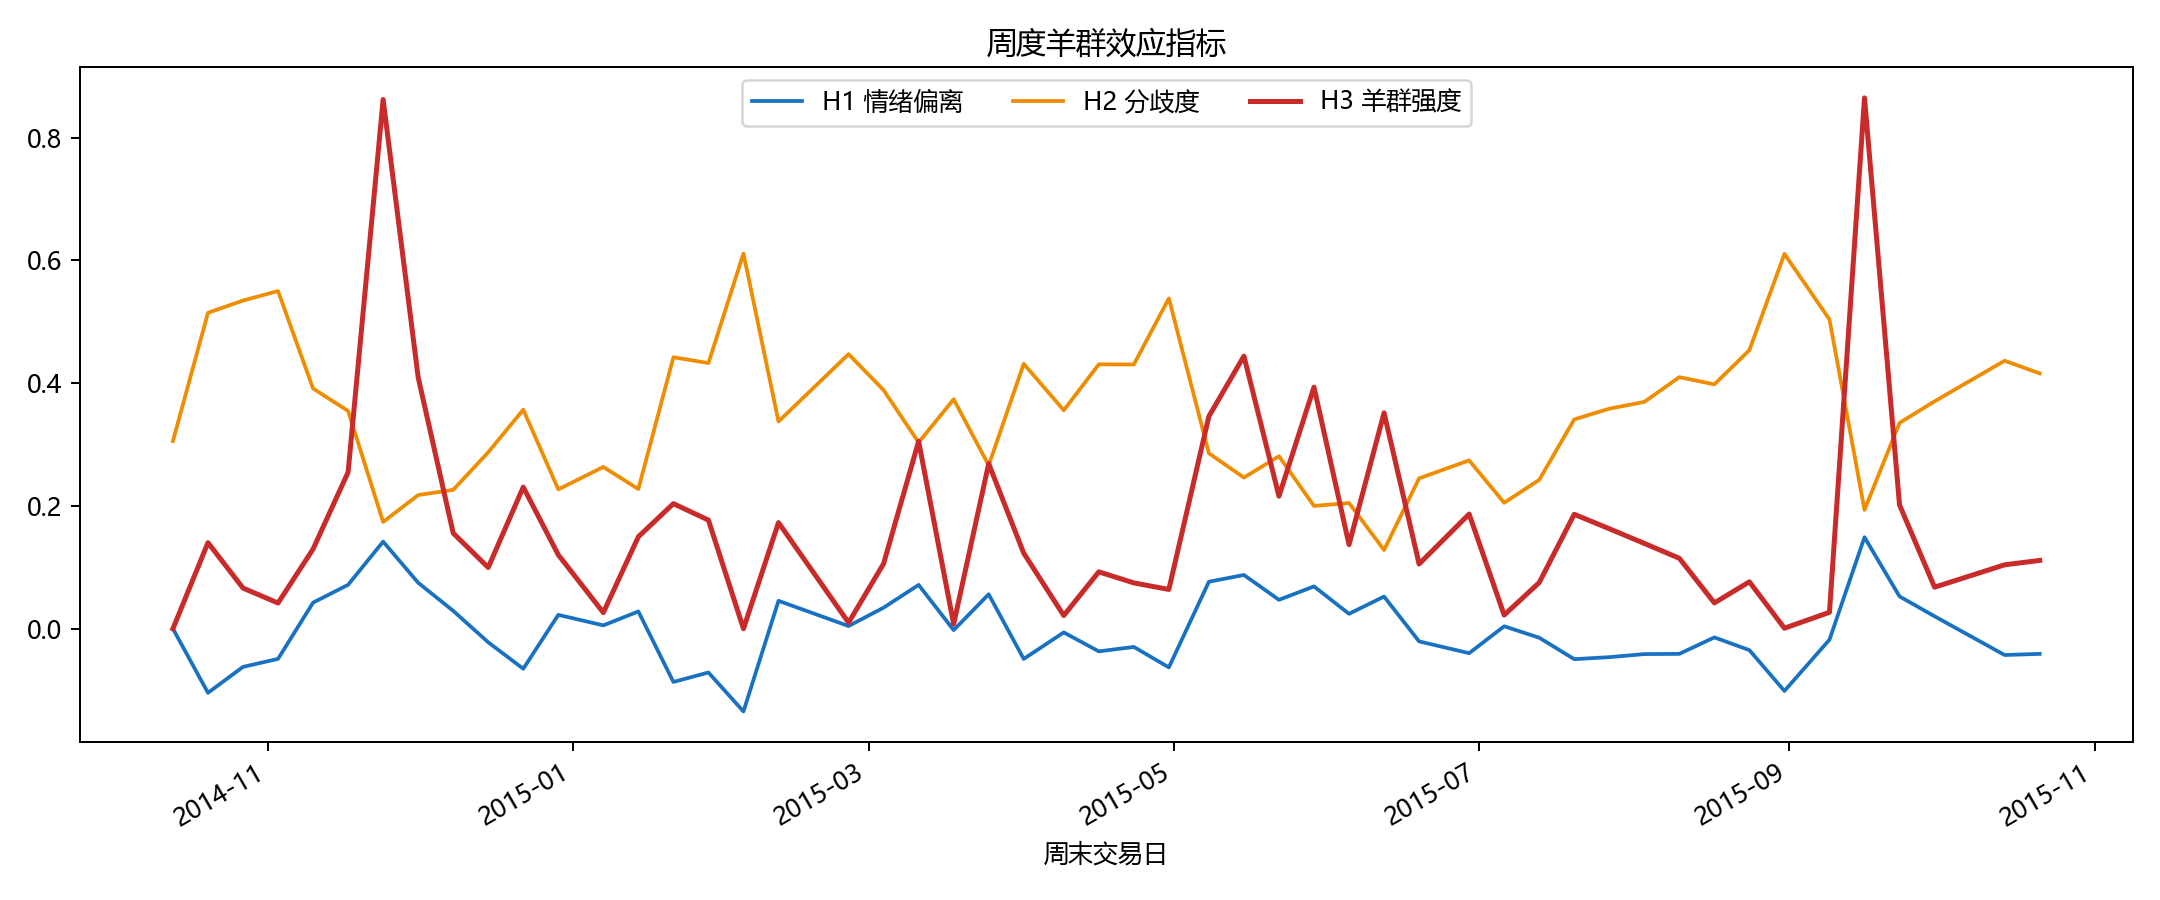
\includegraphics[width=0.92\textwidth]{herd_index_timeseries.png}
    \caption{周度羊群效应指标时序图}
    \label{fig:herd-index-timeseries}
\end{figure}

图 \ref{fig:herd-index-snapshot} 展示了 $P_t$、$E(P_t)$、$H1_t$、$H2_t$ 和 $H3_t$ 的样例结果。首期由于不存在历史 4 周基准，$E(P_t)$ 和 $H1_t$ 为空，后续建模时自动剔除。图 \ref{fig:herd-index-timeseries} 显示，$H3_t$ 并非简单跟随 $P_t$ 上下波动，而是在情绪偏离和单边一致性同时较强时才出现高值，这符合羊群效应指数的设计目标。

\subsection{数据质量分析}

羊群指标的数据质量主要体现在三方面。第一，所有指标均基于交易日过滤后的新闻样本，避免了非交易日文本与价格序列错位。第二，$P_t$ 的分母只使用正负情绪文本，避免中性公告数量过大造成方向性情绪被稀释。第三，$H1_t$ 使用过去 4 周均值作为基准，严格使用历史信息，避免使用未来情绪数据。后续机器学习特征中的滞后项和滚动统计也已先进行 \texttt{shift(1)}，保证预测当周收益时只使用过去已知信息。

\section{实验三：LightGBM 非线性预测与双向传导验证}

\subsection{数据对齐与特征工程}

实验三将实验二输出的周度羊群效应指标与沪深300周收益率按 \texttt{week\_id} 和周末交易日内连接对齐。沪深300周收益率使用每 5 个交易日分组后的最后收盘价计算：

\begin{equation}
Ret_t=\frac{Close_t-Close_{t-1}}{Close_{t-1}}.
\end{equation}

特征工程围绕 $H3_t$ 构造。核心滞后特征包括 \texttt{H3\_lag1} 至 \texttt{H3\_lag5}，分别表示过去 1 至 5 周羊群效应；滚动统计特征包括过去 3 周和 5 周的均值与标准差；时间特征包括月份和季度。所有滚动特征均先对原序列进行 \texttt{shift(1)} 再滚动计算，确保不包含目标周的同期情绪。

\subsection{正向预测模型}

正向模型使用过去的羊群效应特征预测当周沪深300收益率。数据按时间顺序划分，前 80\% 作为训练集，后 20\% 作为测试集，不使用随机划分。模型采用 LightGBM 回归器，参数设置为学习率 0.1、最大深度 3、叶子节点数 7、估计器数量 200，并设置随机种子 42。

\begin{table}[H]
    \centering
    \caption{正向模型测试集指标}
    \label{tab:forward-metrics}
    \begin{tabular}{lr}
        \toprule
        指标 & 数值 \\
        \midrule
        MSE & 0.006118 \\
        MAE & 0.053541 \\
        $R^2$ & -0.2759 \\
        IC（Spearman 秩相关） & 0.2500 \\
        方向命中率 & 44.44\% \\
        测试集样本数 & 9 \\
        \bottomrule
    \end{tabular}
\end{table}

表 \ref{tab:forward-metrics} 表明，正向模型测试集 $R^2$ 为负，说明在当前样本量下，模型样本外预测误差仍高于简单均值基准。IC 为 0.2500，说明预测排序存在一定弱信号，但方向命中率只有 44.44\%，不能认为羊群效应对当周收益具有稳定预测能力。

\begin{figure}[H]
    \centering
    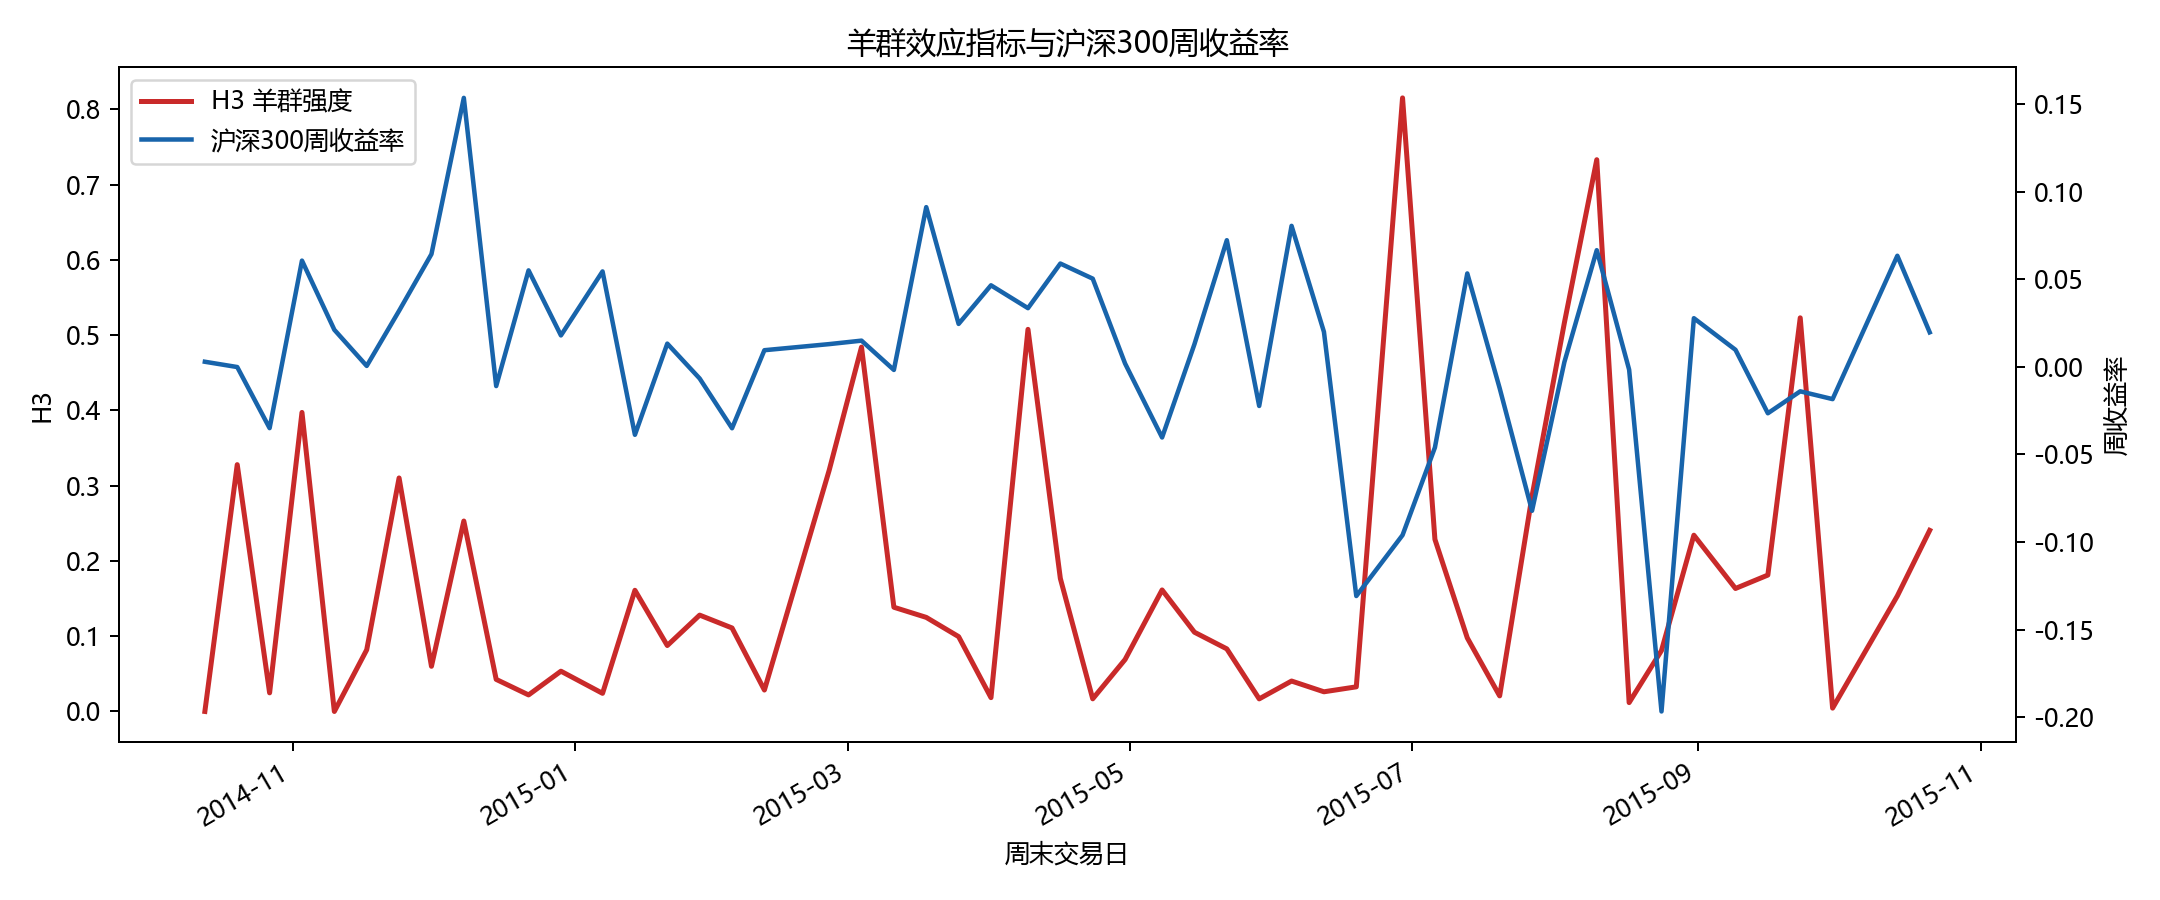
\includegraphics[width=0.92\textwidth]{herd_vs_hs300_return.png}
    \caption{羊群效应指标与沪深300周收益率对比}
    \label{fig:herd-vs-return}
\end{figure}

\begin{figure}[H]
    \centering
    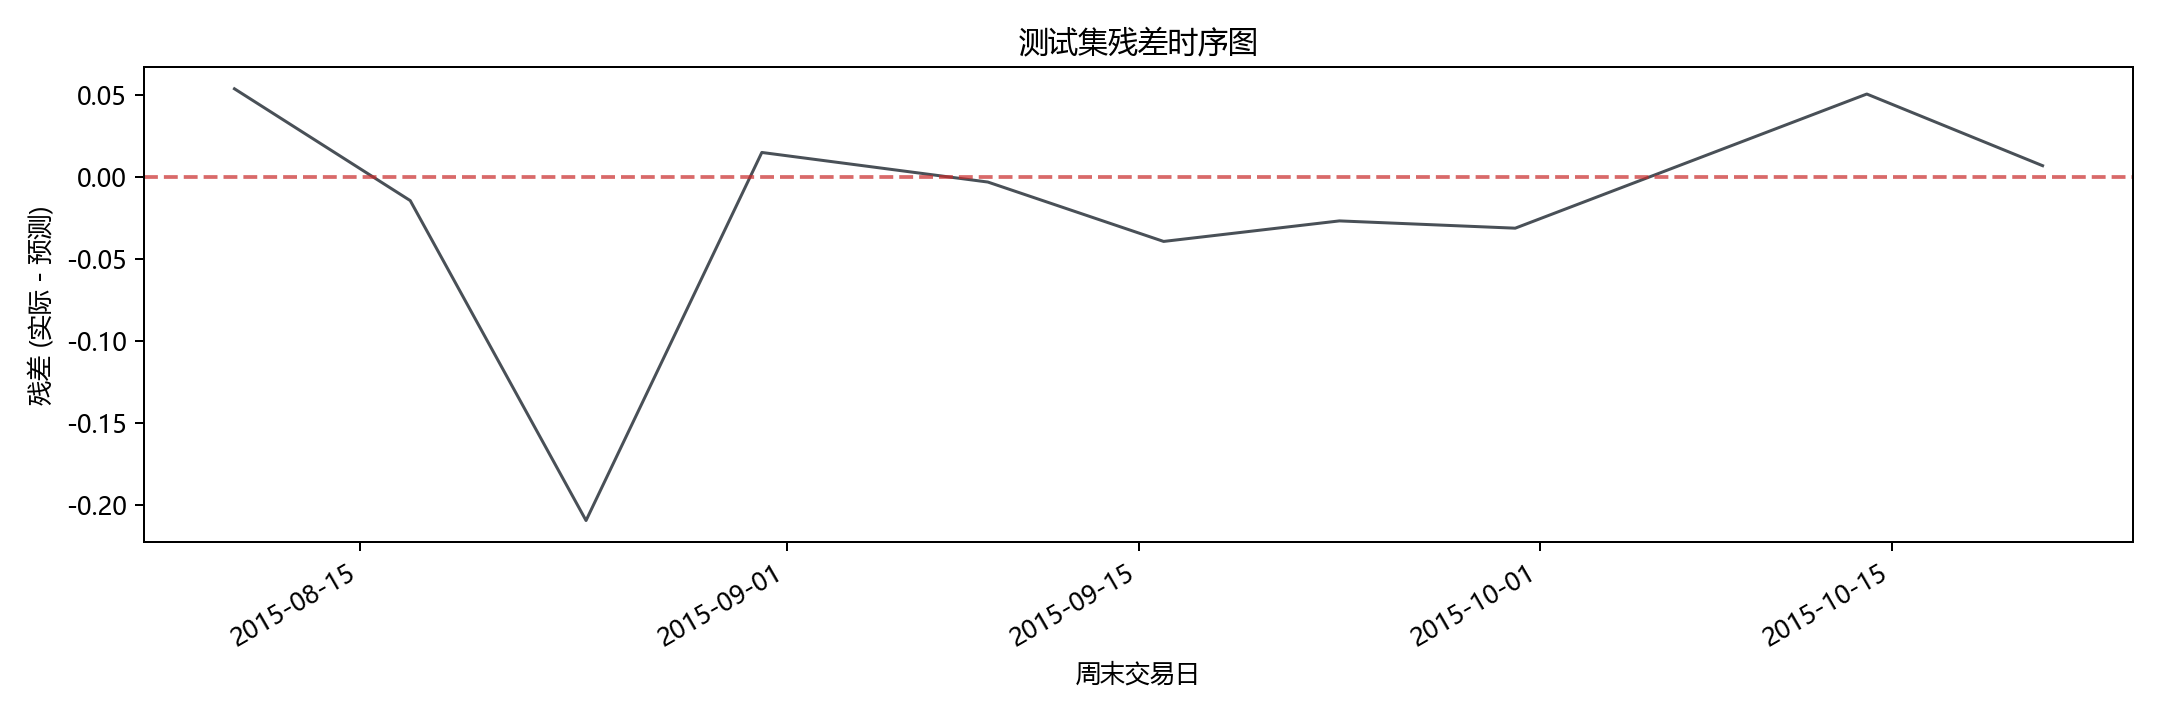
\includegraphics[width=0.82\textwidth]{residual_timeseries.png}
    \caption{正向模型测试集残差时序图}
    \label{fig:residual-timeseries}
\end{figure}

图 \ref{fig:herd-vs-return} 显示，羊群效应与收益率在若干时期存在共同波动，但整体关系并不稳定。图 \ref{fig:residual-timeseries} 显示，测试集残差存在明显波动，说明单独依靠情绪羊群特征难以稳定解释短期指数收益。

\subsection{LightGBM 特征重要性与 SHAP 分析}

为了区分模型内部 gain 重要性和 SHAP 解释，本实验分别输出 \path{lgbm_feature_importance.csv} 和 \path{shap_importance.csv}。LightGBM gain 重要性衡量特征在树分裂中带来的损失下降，SHAP 则从样本层面解释每个特征对预测值的边际贡献。

\begin{figure}[H]
    \centering
    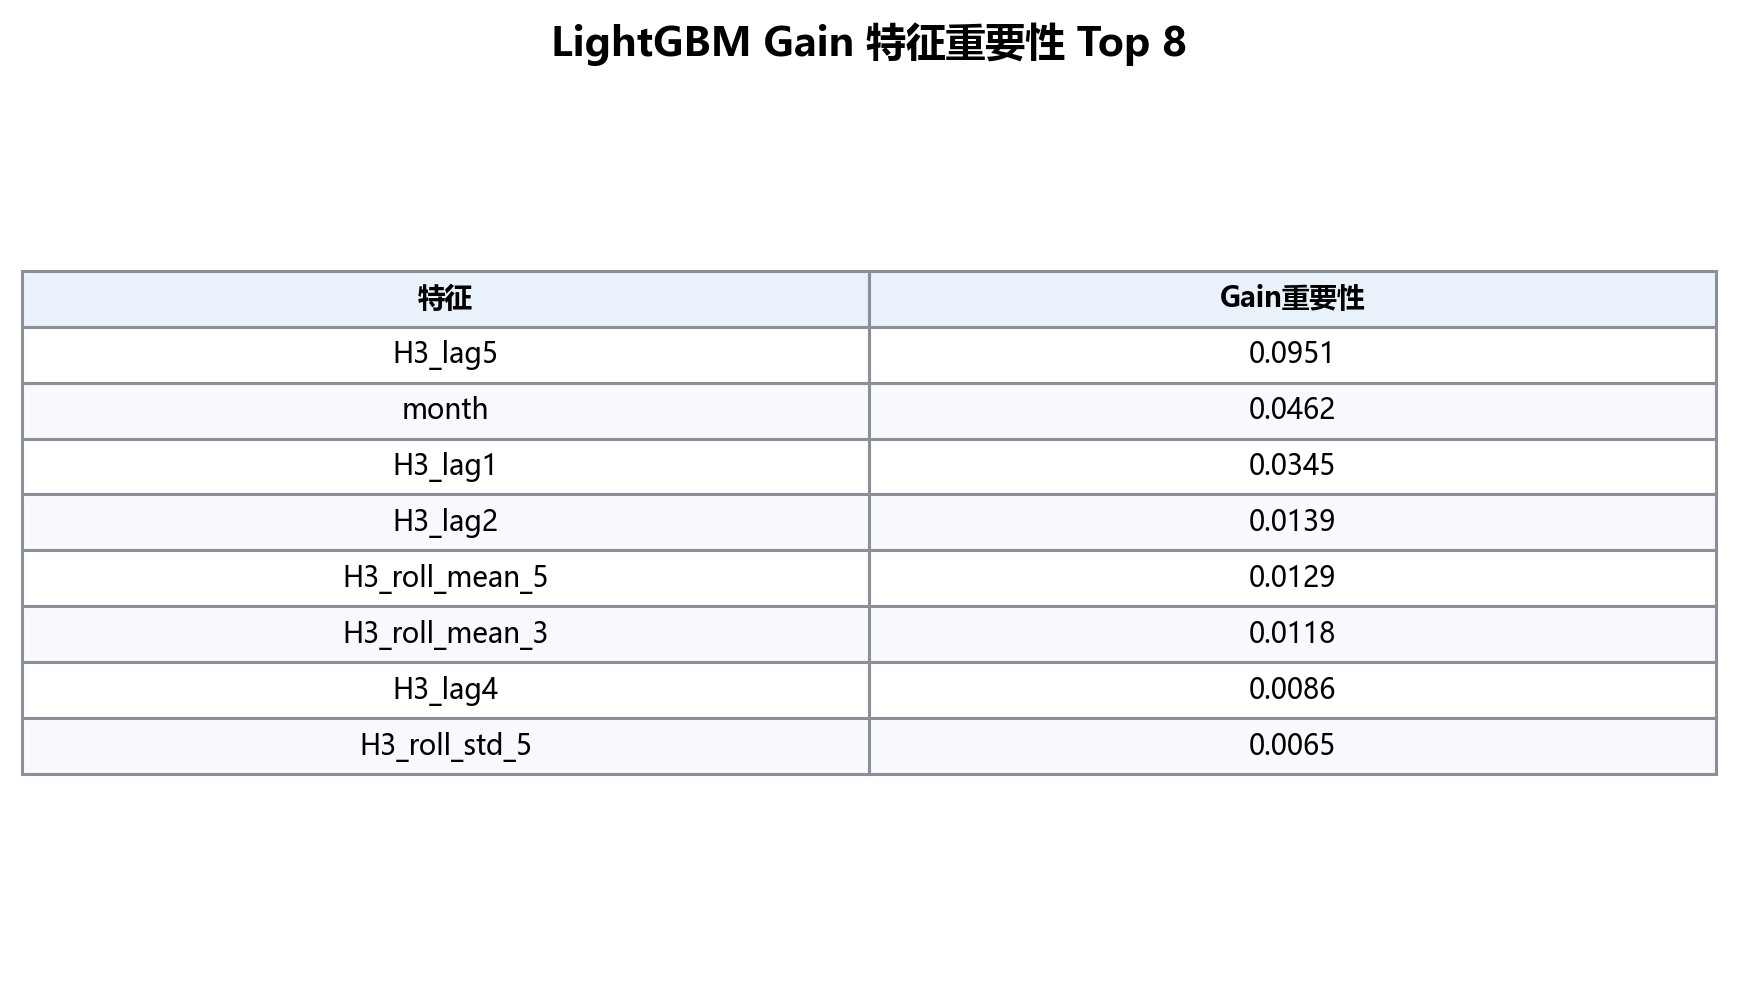
\includegraphics[width=0.82\textwidth]{lgbm_importance_snapshot.png}
    \caption{LightGBM Gain 特征重要性表截图}
    \label{fig:lgbm-importance-snapshot}
\end{figure}

\begin{figure}[H]
    \centering
    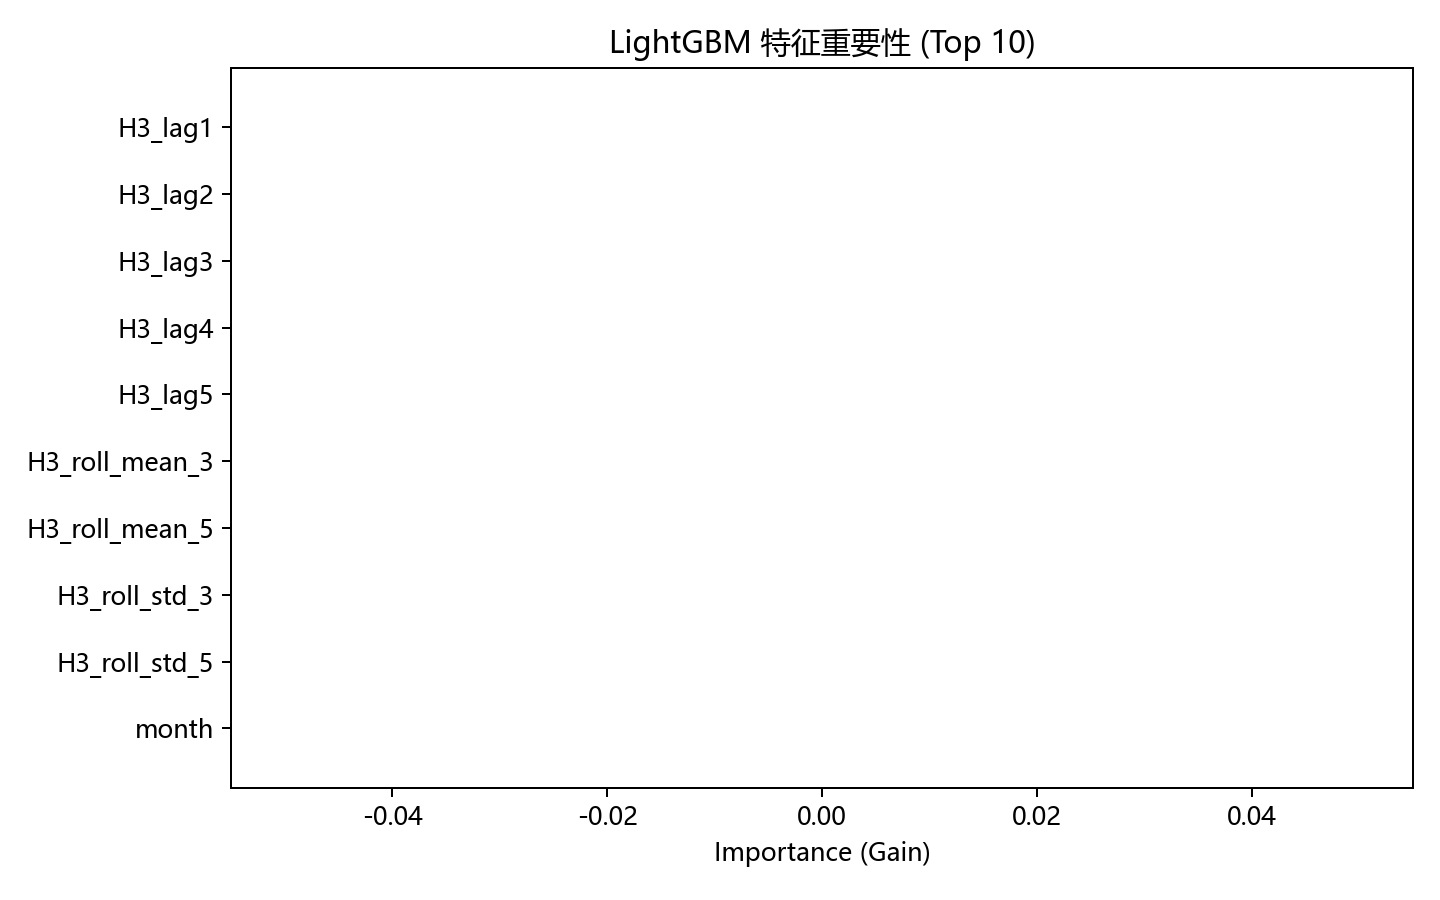
\includegraphics[width=0.78\textwidth]{feature_importance.png}
    \caption{LightGBM Gain 特征重要性图}
    \label{fig:lgbm-importance}
\end{figure}

从图 \ref{fig:lgbm-importance-snapshot} 和图 \ref{fig:lgbm-importance} 可以看出，最重要的羊群效应特征为 \texttt{H3\_lag5}，说明在当前样本中，5 周前的羊群效应对收益预测贡献最大。月份特征也具有较高 gain，说明样本中可能存在阶段性行情或季节性结构，但由于测试集只有 9 条，不能过度解释。

\begin{figure}[H]
    \centering
    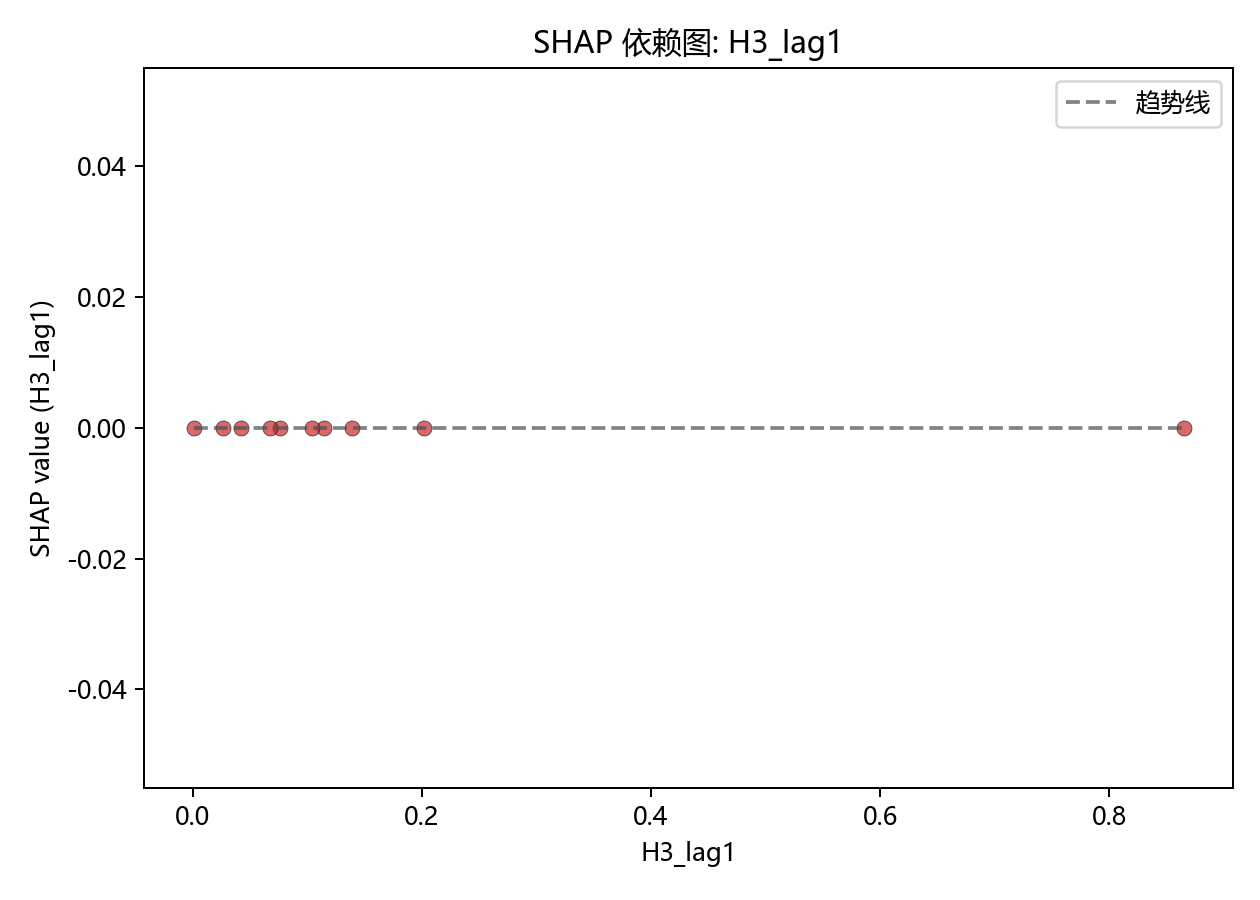
\includegraphics[width=0.78\textwidth]{shap_dependence.png}
    \caption{SHAP 依赖图}
    \label{fig:shap-dependence}
\end{figure}

图 \ref{fig:shap-dependence} 以 SHAP 值展示最重要特征对收益预测的影响。该图的意义不是证明线性显著关系，而是说明 LightGBM 模型如何在测试样本中利用 \texttt{H3\_lag5} 调整预测值。由于样本量较小，SHAP 图更适合作为模型解释证据，而不能单独作为强统计结论。

\subsection{双向传导验证}

为了验证金融反身性，本实验构建两个方向的模型：正向模型使用滞后羊群效应预测收益率，反向模型使用滞后收益率预测羊群效应。反向模型的滚动收益特征同样先进行 \texttt{shift(1)}，避免当周收益泄露。反向方向命中率不再使用 $H3_t$ 的正负号，因为 $H3_t$ 本身非负，而是比较预测 $H3_t$ 相对上一期 $H3_{t-1}$ 的涨跌方向是否正确。

\begin{figure}[H]
    \centering
    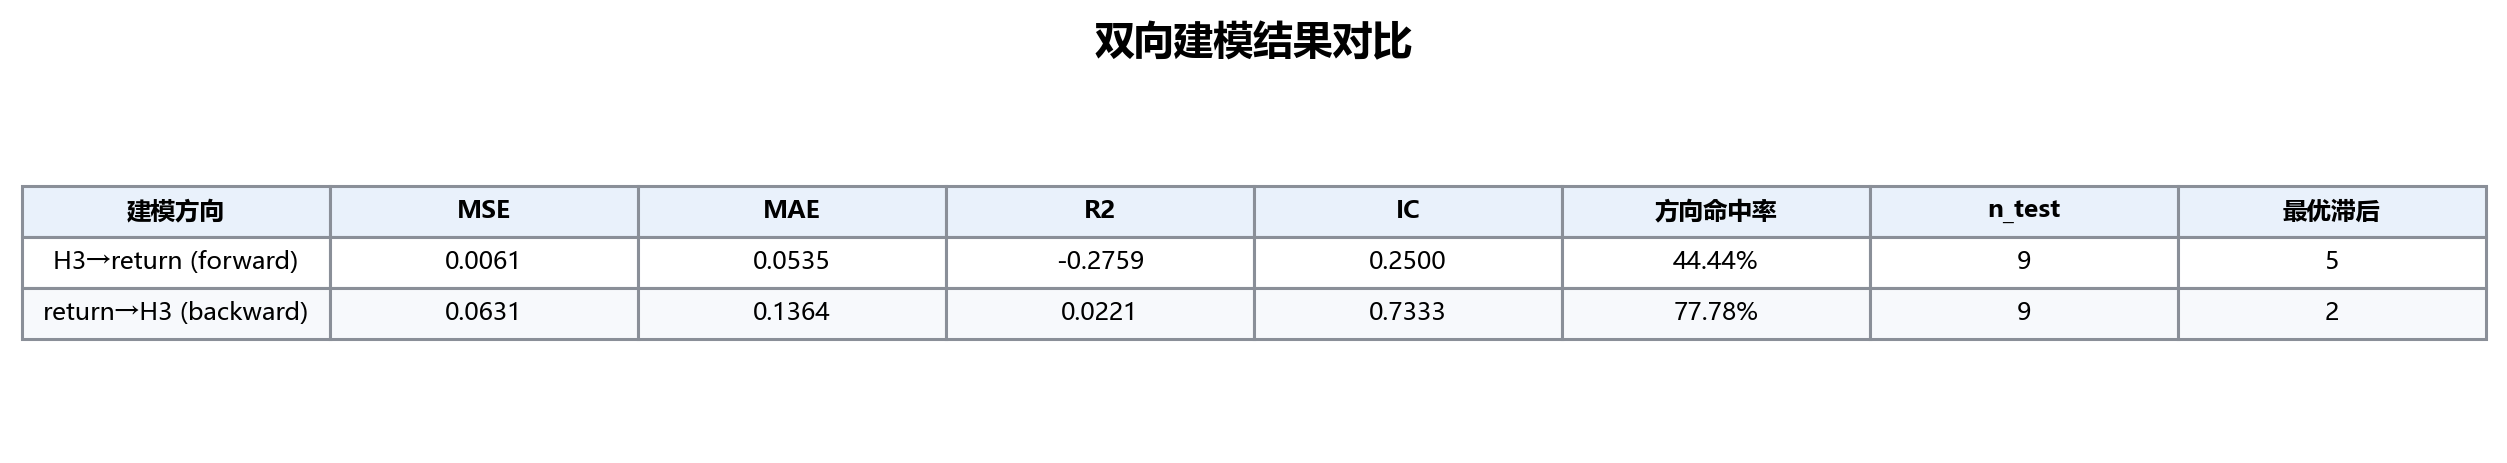
\includegraphics[width=0.90\textwidth]{model_metrics_snapshot.png}
    \caption{双向建模结果表截图}
    \label{fig:model-metrics-snapshot}
\end{figure}

\begin{figure}[H]
    \centering
    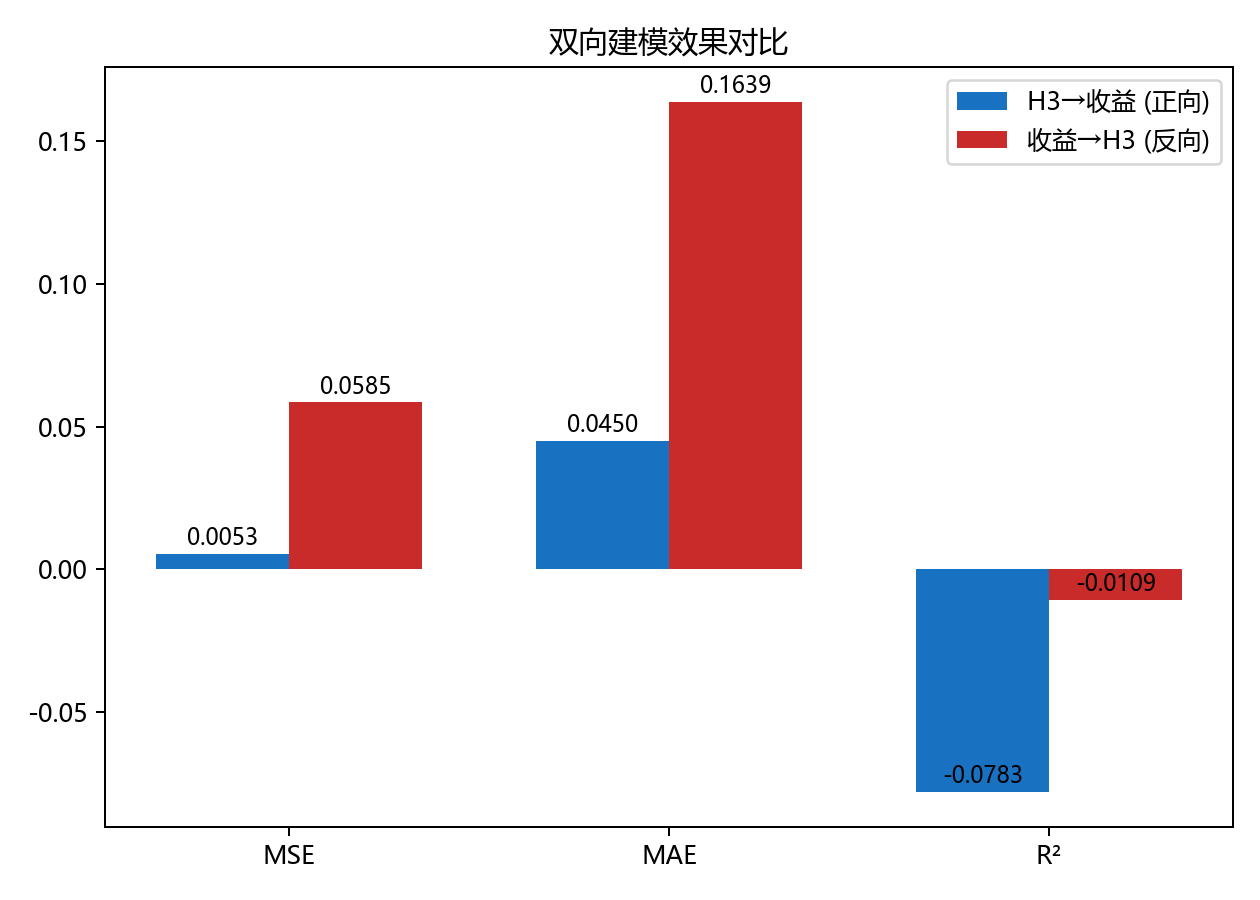
\includegraphics[width=0.76\textwidth]{bidirectional_comparison.png}
    \caption{双向建模效果对比图}
    \label{fig:bidirectional-comparison}
\end{figure}

图 \ref{fig:model-metrics-snapshot} 和图 \ref{fig:bidirectional-comparison} 表明，反向模型测试集 $R^2=0.0221$，高于正向模型的 $R^2=-0.2759$；反向 IC 为 0.7333，也高于正向 IC 0.2500。虽然反向模型解释力仍然较弱，但相对正向模型更稳定，说明当前数据中“市场收益变化影响后续情绪羊群强度”的反馈路径强于“情绪羊群强度预测后续收益”的先行路径。

\section{AI 代码审核与修复记录}

实验指导要求提交 AI 代码审核表。本节记录本次 AI 辅助审查发现的问题、修复方式和验证结果。审核重点不是形式化罗列，而是确认代码是否满足金融时间序列任务中的关键约束。

{\small
\begin{longtable}{@{}L{0.14\textwidth}L{0.24\textwidth}L{0.40\textwidth}L{0.09\textwidth}@{}}
    \caption{AI 代码审核与修复记录}
    \label{tab:ai-audit}\\
    \toprule
    审核项 & 发现问题 & 修复或确认结果 & 状态 \\
    \midrule
    \endfirsthead
    \toprule
    审核项 & 发现问题 & 修复或确认结果 & 状态 \\
    \midrule
    \endhead
    情绪公式 & 检查 $P_t$ 分母是否应包含中性新闻。 & 对照实验公式后确认 $P_t=Positive/(Positive+Negative)$，代码实现正确。 & 通过 \\
    羊群指标 & $H2_t$ 越小表示越一致，若直接乘 $Norm(H2_t)$ 会与解释矛盾。 & 代码采用 $Norm(|H1_t|)\times(1-Norm(H2_t))$，并在代码注释中明确 $H2_t$ 为分歧度。 & 通过 \\
    时序泄露 & 原滚动均值和滚动标准差包含当周 $H3_t$ 或当周收益。 & 已改为先 \texttt{shift(1)} 再滚动，确保特征只使用目标周之前的信息。 & 已修复 \\
    特征重要性 & 原图把 SHAP 平均绝对值误标为 LightGBM Gain。 & 新增 LightGBM gain 明细输出，图表改为真正的 LightGBM gain；SHAP 单独输出。 & 已修复 \\
    反向命中率 & $H3_t$ 非负，直接用符号计算方向准确率会虚高。 & 改为相对上一期 $H3$ 的涨跌方向命中率，结果为 77.78\%。 & 已修复 \\
    可复现性 & 需要验证主流程能从原始数据重新生成结果。 & 已复跑 \texttt{python -m experiment1.main}，BERT 标注 30623 条并生成全部输出。 & 通过 \\
    数据库存储 & 需要确认 CSV 与 SQLite 结果存在。 & SQLite 中周度情绪、羊群指标、建模数据集等核心结果表均存在。 & 通过 \\
    \bottomrule
\end{longtable}
}

\section{运行结果与复现说明}

本实验在 Windows 环境下运行，Python 版本为 3.11.5，主要依赖包括 pandas、numpy、matplotlib、scikit-learn、lightgbm、scipy、xlrd、transformers、torch 和 shap。依赖列表保存在 \path{requirements.txt}。复现实验时，在仓库根目录执行：

\begin{CodeBlock}
python -m experiment1.main
\end{CodeBlock}

程序会自动读取 \path{data/experiment1/raw/} 中的新闻数据和沪深300日度价格数据，生成周度情绪、羊群指标、建模数据、CSV、SQLite 数据库、图表和摘要 JSON。核心输出文件见表 \ref{tab:output-files}。

\begin{longtable}{p{0.34\textwidth}p{0.56\textwidth}}
    \caption{核心输出文件清单}
    \label{tab:output-files}\\
    \toprule
    文件 & 说明 \\
    \midrule
    \endfirsthead
    \toprule
    文件 & 说明 \\
    \midrule
    \endhead
    \path{weekly_sentiment.csv} & 实验一周度情绪指标表。 \\
    \path{weekly_herd_index.csv} & 实验二羊群效应指标表。 \\
    \path{hs300_weekly_return.csv} & 沪深300按 5 个交易日聚合后的周收益表。 \\
    \path{modeling_dataset.csv} & 羊群效应与沪深300收益率对齐后的建模数据。 \\
    \path{feature_engineering.csv} & 滞后特征、滚动统计特征和时间特征数据集。 \\
    \path{lgbm_forward_results.csv} & 正向 LightGBM 测试集预测、真实收益和残差。 \\
    \path{lgbm_feature_importance.csv} & LightGBM gain 特征重要性。 \\
    \path{shap_importance.csv} & SHAP 平均绝对贡献度排序。 \\
    \path{bidirectional_comparison.csv} & 正向与反向建模指标对比。 \\
    \path{experiment1.db} & SQLite 数据库，保存核心结果表。 \\
    \path{summary.json} & 全流程审计、指标、图表和解释摘要。 \\
    \bottomrule
\end{longtable}

\section{实验结论}

第一，实验一已经完成从非结构化金融新闻到结构化周度情绪指标的转换。经过清洗、去重、交易日过滤和 BERT 情绪标注后，30623 条新闻进入周度聚合，生成 51 行周度情绪数据，并同时导出 CSV 和写入 SQLite 数据库。

第二，实验二构造的羊群效应指数能够同时反映情绪偏离和单边一致性。单纯的乐观比例 $P_t$ 不能代表羊群效应，必须结合历史基准和观点分歧度。$H3_t$ 的高值对应“情绪异常且观点一边倒”的时期，符合金融羊群效应的指标逻辑。

第三，实验三表明，在当前小样本条件下，羊群效应对沪深300周收益率的正向预测能力有限。正向模型 $R^2$ 为负，说明其预测误差仍大于均值基准；虽然 \texttt{H3\_lag5} 在 gain 和 SHAP 中均排名靠前，但这只能说明模型使用了该特征，不能证明其具有稳定强预测能力。

第四，反向模型的表现相对更好，说明市场收益对后续情绪和羊群强度的影响更明显。这与金融反身性理论一致：市场涨跌会改变新闻叙事和投资者情绪，进而影响下一阶段的群体行为。当前数据更支持“收益驱动舆情”的反馈路径，而不是“舆情稳定预测收益”的单向路径。

第五，实验仍存在样本规模较小、测试集只有 9 周、情绪模型未针对本数据集重新微调等限制。后续若要增强结论可靠性，应扩展新闻和行情时间跨度，加入成交量、波动率、宏观变量和行业变量，并采用滚动窗口回测检验模型稳定性。

\clearpage
\appendix
\section{完整代码附录}

本附录列出实验一完整核心代码。代码以仓库中的实际文件为准，路径为 \path{experiment1/}。

\subsection{\texorpdfstring{\texttt{config.py}}{config.py}}
\CodeInput{../../experiment1/config.py}

\subsection{\texorpdfstring{\texttt{sentiment.py}}{sentiment.py}}
\CodeInput{../../experiment1/sentiment.py}

\subsection{\texorpdfstring{\texttt{data.py}}{data.py}}
\CodeInput{../../experiment1/data.py}

\subsection{\texorpdfstring{\texttt{analysis.py}}{analysis.py}}
\CodeInput{../../experiment1/analysis.py}

\subsection{\texorpdfstring{\texttt{plots.py}}{plots.py}}
\CodeInput{../../experiment1/plots.py}

\subsection{\texorpdfstring{\texttt{main.py}}{main.py}}
\CodeInput{../../experiment1/main.py}

\end{document}
